% PGSD — Parallelized General Simulation Data
% Reference Manual
% Author: David Krach, University of Stuttgart
% Version 3.2.0

\documentclass[11pt,a4paper,twoside]{article}

% --------------------------------------------------------------------------
% Packages
% --------------------------------------------------------------------------
\usepackage[T1]{fontenc}
\usepackage[utf8]{inputenc}
\usepackage{lmodern}
\usepackage[english]{babel}
\usepackage[margin=2.5cm,top=3cm,bottom=3cm]{geometry}
\usepackage{hyperref}
\usepackage{xcolor}
\usepackage{listings}
\usepackage{booktabs}
\usepackage{array}
\usepackage{longtable}
\usepackage{tabularx}
\usepackage{amsmath}
\usepackage{amssymb}
\usepackage{graphicx}
\usepackage{fancyhdr}
\usepackage{titlesec}
\usepackage{tocloft}
\usepackage{microtype}
\usepackage{parskip}
\usepackage{enumitem}
\usepackage{tikz}
\usetikzlibrary{shapes.geometric,arrows.meta,positioning,fit,backgrounds}

% --------------------------------------------------------------------------
% Colours
% --------------------------------------------------------------------------
\definecolor{pgsdblue}{HTML}{0b3c82}
\definecolor{pgsdgray}{HTML}{4a4a4a}
\definecolor{codebg}{HTML}{f5f5f5}
\definecolor{codefg}{HTML}{2b2b2b}
\definecolor{kwcolor}{HTML}{0033b3}
\definecolor{strcolor}{HTML}{067d17}
\definecolor{cmtcolor}{HTML}{8c8c8c}
\definecolor{typecolor}{HTML}{6e3b6e}

% --------------------------------------------------------------------------
% Hyperref setup
% --------------------------------------------------------------------------
\hypersetup{
    colorlinks  = true,
    linkcolor   = pgsdblue,
    urlcolor    = pgsdblue,
    citecolor   = pgsdblue,
    pdftitle    = {PGSD Reference Manual},
    pdfauthor   = {David Krach},
    pdfsubject  = {Parallelized General Simulation Data},
}

% --------------------------------------------------------------------------
% Listings
% --------------------------------------------------------------------------
\lstdefinestyle{pgsdC}{
    language        = C,
    basicstyle      = \ttfamily\small\color{codefg},
    keywordstyle    = \color{kwcolor}\bfseries,
    stringstyle     = \color{strcolor},
    commentstyle    = \color{cmtcolor}\itshape,
    backgroundcolor = \color{codebg},
    frame           = single,
    framerule       = 0.4pt,
    rulecolor       = \color{pgsdgray!40},
    numbers         = left,
    numberstyle     = \tiny\color{pgsdgray},
    numbersep       = 8pt,
    breaklines      = true,
    showstringspaces= false,
    tabsize         = 4,
    xleftmargin     = 1.5em,
    xrightmargin    = 0.5em,
}

\lstdefinestyle{pgsdPython}{
    language        = Python,
    basicstyle      = \ttfamily\small\color{codefg},
    keywordstyle    = \color{kwcolor}\bfseries,
    stringstyle     = \color{strcolor},
    commentstyle    = \color{cmtcolor}\itshape,
    backgroundcolor = \color{codebg},
    frame           = single,
    framerule       = 0.4pt,
    rulecolor       = \color{pgsdgray!40},
    numbers         = left,
    numberstyle     = \tiny\color{pgsdgray},
    numbersep       = 8pt,
    breaklines      = true,
    showstringspaces= false,
    tabsize         = 4,
    xleftmargin     = 1.5em,
    xrightmargin    = 0.5em,
}

\lstdefinestyle{pgsdBash}{
    language        = bash,
    basicstyle      = \ttfamily\small\color{codefg},
    keywordstyle    = \color{kwcolor},
    commentstyle    = \color{cmtcolor}\itshape,
    backgroundcolor = \color{codebg},
    frame           = single,
    framerule       = 0.4pt,
    rulecolor       = \color{pgsdgray!40},
    breaklines      = true,
    showstringspaces= false,
    xleftmargin     = 1.5em,
    xrightmargin    = 0.5em,
}

% Inline code
\newcommand{\code}[1]{\texttt{#1}}
\newcommand{\chunk}[1]{\texttt{\textcolor{pgsdblue}{#1}}}

% --------------------------------------------------------------------------
% Header / footer
% --------------------------------------------------------------------------
\pagestyle{fancy}
\fancyhf{}
\fancyhead[LE,RO]{\small\thepage}
\fancyhead[LO]{\small\nouppercase{\rightmark}}
\fancyhead[RE]{\small PGSD Reference Manual}
\renewcommand{\headrulewidth}{0.4pt}

% --------------------------------------------------------------------------
% Section formatting
% --------------------------------------------------------------------------
\titleformat{\section}
  {\Large\bfseries\color{pgsdblue}}{\thesection}{1em}{}[\color{pgsdblue}\titlerule]
\titleformat{\subsection}
  {\large\bfseries\color{pgsdblue}}{\thesubsection}{1em}{}
\titleformat{\subsubsection}
  {\normalsize\bfseries\color{pgsdgray}}{\thesubsubsection}{1em}{}

% --------------------------------------------------------------------------
% Note / Warning boxes
% --------------------------------------------------------------------------
\newcommand{\notebox}[1]{%
  \vspace{0.5em}%
  \noindent\colorbox{codebg}{%
    \begin{minipage}{0.97\linewidth}%
      \vspace{0.3em}%
      \textbf{\textcolor{pgsdblue}{Note:}}\ #1%
      \vspace{0.3em}%
    \end{minipage}%
  }%
  \vspace{0.5em}%
}

\newcommand{\warnbox}[1]{%
  \vspace{0.5em}%
  \noindent\colorbox{yellow!20}{%
    \begin{minipage}{0.97\linewidth}%
      \vspace{0.3em}%
      \textbf{\textcolor{red!70!black}{Warning:}}\ #1%
      \vspace{0.3em}%
    \end{minipage}%
  }%
  \vspace{0.5em}%
}

% ==========================================================================
% Document
% ==========================================================================
\begin{document}

% --------------------------------------------------------------------------
% Title page
% --------------------------------------------------------------------------
\begin{titlepage}
  \begin{center}
    \vspace*{2cm}
    {\Huge\bfseries\color{pgsdblue} PGSD}\\[0.4em]
    {\Large\color{pgsdgray} Parallelized General Simulation Data}\\[0.2em]
    {\large\color{pgsdgray} Reference Manual}\\[2em]
    \rule{0.5\textwidth}{1pt}\\[2em]
    {\large Version 3.2.0}\\[1em]
    {\normalsize David Krach}\\
    {\small\color{pgsdgray} Institute of Applied Mechanics\\
    University of Stuttgart}\\[0.5em]
    {\small\href{mailto:david.krach@mib.uni-stuttgart.de}{david.krach@mib.uni-stuttgart.de}}\\[2em]
    \rule{0.5\textwidth}{0.4pt}\\[1em]
    {\small Based on the GSD library by the Glotzer Group, University of Michigan.\\
    Released under the BSD 2-Clause License.}\\[3em]
    {\small\today}
  \end{center}
\end{titlepage}

% --------------------------------------------------------------------------
% Abstract
% --------------------------------------------------------------------------
\begin{abstract}
\noindent
PGSD (Parallelized General Simulation Data) is an MPI-parallel file I/O library
for Smoothed Particle Hydrodynamics (SPH) simulation output.  It is a fork of
the GSD library from the Glotzer Group (University of Michigan) that replaces
serial POSIX I/O with collective MPI-IO, enabling all simulation ranks to write
their particle partitions directly and concurrently without gathering data to the
root process.

This manual describes the PGSD file format, the HOOMD schema with its SPH
extensions, the Python and C programming interfaces, and the internal MPI
parallel I/O design.
\end{abstract}

\tableofcontents
\clearpage

% ==========================================================================
\section{Introduction}
% ==========================================================================

\subsection{Overview}

PGSD stores simulation trajectories as a sequence of \emph{frames}.  Each frame
holds a set of named, typed data \emph{chunks} such as particle positions,
velocities, or scalar fields.  The file format is binary and optimised for
high-performance write throughput from MPI-parallel simulations.

PGSD preserves the on-disk format of GSD so that existing GSD-compatible tools
(OVITO, gsd-vmd, freud) can read PGSD output files without modification.

\subsection{Design goals}

\begin{itemize}[noitemsep]
  \item Eliminate the serial gather-to-root bottleneck present in the original
        GSD library.
  \item Every MPI rank writes its own particle partition directly using
        \code{MPI\_File\_write\_at}.
  \item Keep metadata (index entries, chunk namelist) consistent by managing
        them exclusively on rank~0 while collecting per-rank sizes via
        \code{MPI\_Allgather}.
  \item Maintain binary compatibility with GSD v1/v2 files so post-processing
        tools require no modification.
\end{itemize}

\subsection{Differences from GSD}

\begin{center}
\begin{tabular}{lll}
  \toprule
  Feature & GSD & PGSD \\
  \midrule
  File I/O        & POSIX (serial)          & MPI-IO (parallel)           \\
  Index / namelist & root only              & root only (gathered)         \\
  Particle data   & gathered to root        & each rank writes its share   \\
  Particle order  & sorted by tag           & unsorted (rank order)        \\
  Fields per step & only changed fields     & all fields, every step       \\
  File size       & minimal                 & larger                       \\
  \bottomrule
\end{tabular}
\end{center}

Because particles are \emph{not} sorted and all fields are written every
timestep, PGSD files are larger than equivalent GSD files.  This is an explicit
trade-off for write throughput in massively parallel runs.

\subsection{Repository layout}

\begin{center}
\begin{tabular}{ll}
  \toprule
  Path & Description \\
  \midrule
  \code{pgsd/pgsd.c} & MPI-IO C implementation \\
  \code{pgsd/pgsd.h} & C public API header \\
  \code{pgsd/fl.pyx} & Cython wrapper (Python file layer) \\
  \code{pgsd/hoomd.py} & HOOMD schema Python interface \\
  \code{pgsd/pypgsd.py} & Pure Python read-only reader \\
  \code{pgsd/libpgsd.pxd} & Cython C declarations \\
  \code{scripts/} & Benchmark utilities \\
  \code{pgsd/test/} & Unit tests \\
  \bottomrule
\end{tabular}
\end{center}

% ==========================================================================
\section{Installation}
% ==========================================================================

\subsection{Prerequisites}

\begin{center}
\begin{tabular}{lll}
  \toprule
  Dependency & Minimum version & Purpose \\
  \midrule
  MPI (OpenMPI or MPICH) & 4.0 / 3.4 & Parallel I/O \\
  CMake                  & 3.14       & Build system \\
  Python                 & 3.8        & Python bindings \\
  Cython                 & 0.29       & Compiles \code{fl.pyx} \\
  NumPy                  & 1.18       & Array interface \\
  mpi4py                 & 3.0        & MPI from Python \\
  \bottomrule
\end{tabular}
\end{center}

\subsection{Build from source}

\begin{lstlisting}[style=pgsdBash]
cd pgsd-3.2.0
mkdir build && cd build

# Pass MPI compiler wrappers explicitly
CC=/usr/bin/mpicc CXX=/usr/bin/mpicxx cmake ..
make -j$(nproc)
\end{lstlisting}

When using a conda environment:

\begin{lstlisting}[style=pgsdBash]
conda activate pgsd-env
export CMAKE_PREFIX_PATH=$CONDA_PREFIX
CC=$CONDA_PREFIX/bin/mpicc CXX=$CONDA_PREFIX/bin/mpicxx cmake ..
make -j$(nproc)
\end{lstlisting}

After building, add the build directory to \code{PYTHONPATH}:

\begin{lstlisting}[style=pgsdBash]
export PYTHONPATH=/path/to/pgsd-3.2.0/build:$PYTHONPATH
python3 -c "import pgsd.fl; print('pgsd OK')"
\end{lstlisting}

\subsection{Minimal conda environment}

\begin{lstlisting}[style=pgsdBash]
conda create -n pgsd-env python=3.10 cython numpy mpi4py cmake \
      openmpi -c conda-forge
conda activate pgsd-env
\end{lstlisting}

% ==========================================================================
\section{File Format Specification}
\label{sec:fileformat}
% ==========================================================================

\subsection{Overview}

A PGSD file is a binary file consisting of four logical blocks:

\begin{enumerate}[noitemsep]
  \item \textbf{Header block} (256~bytes) — magic number, schema, version,
        and pointers to the index and namelist blocks.
  \item \textbf{Namelist block} — flat array of null-terminated chunk name
        strings.
  \item \textbf{Index block} — array of 32-byte \code{pgsd\_index\_entry}
        structs, one per written chunk.
  \item \textbf{Data chunks} — raw binary data, one per (frame, name) pair.
\end{enumerate}

PGSD files are binary-compatible with GSD v1 and v2 files.  The magic number
is shared (\texttt{0x65DF65DF65DF65DF}).

\subsection{Header block}

The header occupies the first 256~bytes:

\begin{lstlisting}[style=pgsdC]
struct pgsd_header {
    uint64_t magic;                    /* 0x65DF65DF65DF65DF       */
    uint64_t index_location;           /* file offset of index     */
    uint64_t index_allocated_entries;  /* capacity of index block  */
    uint64_t namelist_location;        /* file offset of namelist  */
    uint64_t namelist_allocated_entries;
    uint32_t schema_version;           /* 0xMMMMmmmm => MMMM.mmmm  */
    uint32_t pgsd_version;             /* 0xMMMMmmmm => MMMM.mmmm  */
    char     application[64];          /* null-terminated string   */
    char     schema[64];               /* null-terminated string   */
    char     reserved[80];
};
\end{lstlisting}

All offsets are absolute byte positions from the start of the file.  Version
numbers encode major and minor parts as \texttt{(major << 16) | minor}.

\subsection{Index block}

The index maps (frame, name) pairs to their data chunks.  Each 32-byte entry:

\begin{lstlisting}[style=pgsdC]
struct pgsd_index_entry {
    uint64_t frame;    /* frame index (0-based)                    */
    uint64_t N;        /* number of rows in the data matrix        */
    int64_t  location; /* byte offset of the data chunk in file    */
    uint32_t M;        /* number of columns in the data matrix     */
    uint16_t id;       /* name index in the namelist               */
    uint8_t  type;     /* element type (see Table below)           */
    uint8_t  flags;    /* reserved, must be 0                      */
};
\end{lstlisting}

Element type codes:

\begin{center}
\begin{tabular}{clcl}
  \toprule
  Code & C type & Code & C type \\
  \midrule
  1 & \code{uint8}  & 6 & \code{int16}  \\
  2 & \code{uint16} & 7 & \code{int32}  \\
  3 & \code{uint32} & 8 & \code{int64}  \\
  4 & \code{uint64} & 9 & \code{float32}\\
  5 & \code{int8}   & 10 & \code{float64}\\
  \bottomrule
\end{tabular}
\end{center}

In v2 files, the index is kept sorted by (frame, id).  A binary search is used
to locate entries.  In v1 files, entries are in insertion order and a linear
scan finds the correct entry.

An entry with \code{location == 0} marks the end of the used portion of the
index.  When the index fills up, a new, larger block is allocated at the end of
the file and all entries are rewritten there.

\subsection{Namelist block}

The namelist maps integer \emph{ids} (stored in index entries) to human-readable
chunk names.  Each name is a null-terminated UTF-8 string:

\begin{itemize}[noitemsep]
  \item \textbf{v1 files:} each entry occupies exactly 64~bytes.
  \item \textbf{v2 files:} entries are variable length, separated by
        \texttt{0x00} bytes.
\end{itemize}

The first entry that begins with \texttt{0x00} marks the end of the list.  Up
to 65\,535 distinct chunk names are supported per file.

\subsection{Data chunks}

A data chunk is a contiguous sequence of bytes storing an $N \times M$ array of
elements of a given type.  For index entry \code{e}, the data starts at byte
offset \code{e.location} and occupies
$\code{e.N} \times \code{e.M} \times \text{sizeof(type)}$~bytes.

\subsection{File format limits}

\begin{center}
\begin{tabular}{ll}
  \toprule
  Limit & Value \\
  \midrule
  Maximum file size     & filesystem / 64-bit address space \\
  Chunk names           & up to 65\,535 distinct names per file \\
  Chunk name length     & v1: 63 bytes; v2: unlimited \\
  Application/schema name & 63 characters \\
  Array dimensions      & $N \times M$, $N$: 64-bit, $M$: 32-bit \\
  \bottomrule
\end{tabular}
\end{center}

% ==========================================================================
\section{HOOMD Schema}
\label{sec:hoomd}
% ==========================================================================

\subsection{Overview}

The \texttt{hoomd} schema stores the complete state of a HOOMD-blue simulation.
PGSD extends the standard HOOMD schema with additional SPH-specific particle
fields.

\begin{center}
\begin{tabular}{ll}
  \toprule
  Schema name & \texttt{hoomd} \\
  Schema version & 1.0 \\
  \bottomrule
\end{tabular}
\end{center}

When a chunk is absent from frame $i$, the reader falls back to the value from
frame~0; if absent from frame~0 as well, the default value is used.

\subsection{Configuration chunks}

\begin{longtable}{p{5.5cm}p{1.8cm}p{1.5cm}p{2.5cm}p{1.8cm}}
  \toprule
  Name & Type & Size & Default & Units \\
  \midrule\endhead
  \chunk{configuration/step}       & uint64 & 1$\times$1 & 0         & number \\
  \chunk{configuration/dimensions} & uint8  & 1$\times$1 & 3         & number \\
  \chunk{configuration/box}        & float  & 6$\times$1 & [1,1,1,0,0,0] & varied \\
  \bottomrule
\end{longtable}

\paragraph{configuration/box} encodes the simulation box as
$[l_x, l_y, l_z, xy, xz, yz]$ where $l_{x,y,z}$ are box lengths and $xy$,
$xz$, $yz$ are the tilt factors of the triclinic cell.

\subsection{Standard particle data chunks}

All per-particle arrays have $N$ rows where $N = $ \chunk{particles/N}.

\begin{longtable}{p{5.5cm}p{1.8cm}p{1.5cm}p{2.2cm}p{1.8cm}}
  \toprule
  Name & Type & Size & Default & Units \\
  \midrule\endhead
  \chunk{particles/N}              & uint32 & 1$\times$1 & 0      & number \\
  \chunk{particles/types}          & int8   & $N_T\times M$ & [\texttt{'A'}] & UTF-8 \\
  \chunk{particles/typeid}         & uint32 & $N\times$1 & 0      & number \\
  \chunk{particles/type\_shapes}   & int8   & $N_T\times M$ & \{\} & UTF-8/JSON \\
  \chunk{particles/mass}           & float  & $N\times$1 & 1.0    & mass \\
  \chunk{particles/charge}         & float  & $N\times$1 & 0.0    & charge \\
  \chunk{particles/diameter}       & float  & $N\times$1 & 1.0    & length \\
  \chunk{particles/body}           & int32  & $N\times$1 & $-1$   & number \\
  \chunk{particles/moment\_inertia}& float  & $N\times$3 & 0,0,0  & mass$\cdot$length$^2$ \\
  \chunk{particles/position}       & float  & $N\times$3 & 0,0,0  & length \\
  \chunk{particles/orientation}    & float  & $N\times$4 & 1,0,0,0 & quaternion \\
  \chunk{particles/velocity}       & float  & $N\times$3 & 0,0,0  & length/time \\
  \chunk{particles/angmom}         & float  & $N\times$4 & 0,0,0,0 & quaternion \\
  \chunk{particles/image}          & int32  & $N\times$3 & 0,0,0  & number \\
  \bottomrule
\end{longtable}

\subsection{SPH extension chunks}
\label{sec:sph-chunks}

The following chunks are added by PGSD to support SPH simulations.  They follow
the same chunk naming convention as the standard particle data.

\begin{longtable}{p{5.5cm}p{1.8cm}p{1.5cm}p{2.2cm}p{1.8cm}}
  \toprule
  Name & Type & Size & Default & Units \\
  \midrule\endhead
  \chunk{particles/slength}    & float & $N\times$1 & 1.0     & length \\
  \chunk{particles/density}    & float & $N\times$1 & 0.0     & mass/volume \\
  \chunk{particles/pressure}   & float & $N\times$1 & 0.0     & pressure \\
  \chunk{particles/energy}     & float & $N\times$1 & 0.0     & energy/mass \\
  \chunk{particles/auxiliary1} & float & $N\times$3 & 0,0,0   & user-defined \\
  \chunk{particles/auxiliary2} & float & $N\times$3 & 0,0,0   & user-defined \\
  \chunk{particles/auxiliary3} & float & $N\times$3 & 0,0,0   & user-defined \\
  \chunk{particles/auxiliary4} & float & $N\times$3 & 0,0,0   & user-defined \\
  \bottomrule
\end{longtable}

\paragraph{particles/slength}
Smoothing length $h$ of each SPH particle.  This value defines the kernel
support radius and may vary per particle to achieve adaptive resolution.

\paragraph{particles/density}
Particle density $\rho$.  In weakly compressible SPH this is computed from
the continuity equation or estimated from the kernel sum over neighbours.

\paragraph{particles/pressure}
Particle pressure $p$.  Typically derived from the density via an equation
of state, e.g.\ the Tait equation for weakly compressible flow.

\paragraph{particles/energy}
Specific internal energy $e$.  Used in thermal or compressible SPH
formulations.

\paragraph{particles/auxiliary1--4}
Four generic 3-component float vectors available for user-defined quantities
such as acceleration, surface normal, or intermediate values.  Their physical
interpretation is application-defined.

\subsection{Bond topology chunks}

\begin{longtable}{p{5.5cm}p{1.8cm}p{1.5cm}p{2.2cm}p{1.8cm}}
  \toprule
  Name & Type & Size & Default & Units \\
  \midrule\endhead
  \chunk{bonds/N}        & uint32 & 1$\times$1 & 0 & number \\
  \chunk{bonds/types}    & int8   & $N_T\times M$ & & UTF-8 \\
  \chunk{bonds/typeid}   & uint32 & $N\times$1 & 0 & number \\
  \chunk{bonds/group}    & uint32 & $N\times$2 & 0,0 & number \\
  \bottomrule
\end{longtable}

\subsection{Constraint chunks}

\begin{longtable}{p{5.5cm}p{1.8cm}p{1.5cm}p{2.2cm}p{1.8cm}}
  \toprule
  Name & Type & Size & Default & Units \\
  \midrule\endhead
  \chunk{constraints/N}      & uint32 & 1$\times$1 & 0 & number \\
  \chunk{constraints/value}  & float  & $N\times$1 & 0 & length \\
  \chunk{constraints/group}  & uint32 & $N\times$2 & 0,0 & number \\
  \bottomrule
\end{longtable}

\subsection{Logged data chunks}

Arbitrary quantities can be stored under the \texttt{log/} prefix:

\begin{center}
\begin{tabular}{lll}
  \toprule
  Prefix & Example & Meaning \\
  \midrule
  \chunk{log/} & \chunk{log/value/potential\_energy} & scalar or global quantity \\
  \chunk{log/particles/} & \chunk{log/particles/net\_force} & per-particle array \\
  \chunk{log/bonds/} & \chunk{log/bonds/potential\_energy} & per-bond array \\
  \bottomrule
\end{tabular}
\end{center}

% ==========================================================================
\section{Python API}
\label{sec:python}
% ==========================================================================

Three Python modules are provided:

\begin{center}
\begin{tabular}{ll}
  \toprule
  Module & Description \\
  \midrule
  \code{pgsd.fl}       & Low-level Cython wrapper; creates, reads, writes files \\
  \code{pgsd.hoomd}    & High-level HOOMD schema interface \\
  \code{pgsd.pypgsd}   & Pure Python read-only reader \\
  \bottomrule
\end{tabular}
\end{center}

All modules emit log messages via the standard \code{logging} module.  Enable
debug output with:

\begin{lstlisting}[style=pgsdPython]
import logging
logging.basicConfig(level=logging.DEBUG)
\end{lstlisting}

% --------------------------------------------------------------------------
\subsection{pgsd.fl — File Layer}
\label{sec:fl}
% --------------------------------------------------------------------------

\subsubsection{Opening files: \texttt{pgsd.fl.open}}

\begin{lstlisting}[style=pgsdPython]
pgsd.fl.open(name, mode, application='', schema='', schema_version=[1,0])
\end{lstlisting}

Returns a \code{PGSDFile} object.  \code{mode} must be one of:

\begin{center}
\begin{tabular}{cl}
  \toprule
  Mode & Description \\
  \midrule
  \texttt{'r'}  & Open existing file read-only \\
  \texttt{'r+'} & Open existing file for reading and writing \\
  \texttt{'w'}  & Create or overwrite a file \\
  \texttt{'x'}  & Create exclusively; raise \code{FileExistsError} if exists \\
  \texttt{'a'}  & Open or create for reading and writing \\
  \bottomrule
\end{tabular}
\end{center}

\warnbox{Opening a file in \texttt{'w'} mode overwrites any existing file with
that name.}

\notebox{All MPI ranks must call \code{pgsd.fl.open} collectively.}

\subsubsection{PGSDFile class}

\paragraph{Properties}

\begin{center}
\begin{tabular}{lll}
  \toprule
  Property & Type & Description \\
  \midrule
  \code{name}           & str             & File path \\
  \code{mode}           & str             & Open mode \\
  \code{nframes}        & int             & Number of frames \\
  \code{pgsd\_version}  & (int, int)      & File layer version (major, minor) \\
  \code{schema\_version}& (int, int)      & Schema version (major, minor) \\
  \code{schema}         & str             & Schema name \\
  \code{application}    & str             & Application name \\
  \bottomrule
\end{tabular}
\end{center}

\paragraph{Methods}

\begin{center}
\begin{tabular}{p{7cm}p{7cm}}
  \toprule
  Signature & Description \\
  \midrule
  \code{close(write\_all=True)} & Flush and close the file \\
  \code{end\_frame(write\_all=True)} & Commit current frame and advance counter \\
  \code{flush(write\_all=True)} & Flush write buffer to disk without ending frame \\
  \code{write\_chunk(name, data, offset, write\_all)} & Write a numpy array as a named chunk \\
  \code{read\_chunk(frame, name, N=0, M=0, offset=0, r\_all=False)} & Read a chunk as numpy array \\
  \code{chunk\_exists(frame, name, write\_all=False)} & Test chunk existence \\
  \code{find\_matching\_chunk\_names(match, write\_all=False)} & List chunk names starting with \code{match} \\
  \code{truncate()} & Remove all data, preserve schema \\
  \bottomrule
\end{tabular}
\end{center}

The boolean \code{write\_all} flag controls whether the call is collective
(all ranks participate) or root-only.  Pass \code{write\_all=False} during read
operations when only the root rank processes the result.

\subsubsection{File layer examples}

\paragraph{Create a file and write two frames:}

\begin{lstlisting}[style=pgsdPython]
import pgsd.fl
import numpy

f = pgsd.fl.open(name='simulation.gsd', mode='w',
                 application='my-sph-code', schema='hoomd',
                 schema_version=[1, 0])

# Frame 0
f.write_chunk('particles/N',
              numpy.array([1000], dtype=numpy.uint32))
f.write_chunk('particles/position',
              numpy.random.rand(1000, 3).astype(numpy.float32))
f.write_chunk('particles/velocity',
              numpy.zeros((1000, 3), dtype=numpy.float32))
f.end_frame()

# Frame 1
f.write_chunk('particles/N',
              numpy.array([1000], dtype=numpy.uint32))
f.write_chunk('particles/position',
              numpy.random.rand(1000, 3).astype(numpy.float32))
f.end_frame()

f.close()
\end{lstlisting}

\paragraph{Read a specific chunk from a specific frame:}

\begin{lstlisting}[style=pgsdPython]
f = pgsd.fl.open(name='simulation.gsd', mode='r')
if f.chunk_exists(frame=0, name='particles/position'):
    pos = f.read_chunk(frame=0, name='particles/position')
    # pos.shape == (N, 3), dtype float32
print(f.nframes)
f.close()
\end{lstlisting}

\paragraph{Context manager usage:}

\begin{lstlisting}[style=pgsdPython]
with pgsd.fl.open(name='simulation.gsd', mode='r') as f:
    pos = f.read_chunk(frame=5, name='particles/position')
\end{lstlisting}

% --------------------------------------------------------------------------
\subsection{pgsd.hoomd — HOOMD Schema Interface}
\label{sec:hoomd-py}
% --------------------------------------------------------------------------

\subsubsection{Opening trajectories: \texttt{pgsd.hoomd.open}}

\begin{lstlisting}[style=pgsdPython]
pgsd.hoomd.open(name, mode='r')
\end{lstlisting}

Returns a \code{HOOMDTrajectory} object wrapping a PGSD file with the
\texttt{hoomd} schema.

\subsubsection{HOOMDTrajectory class}

\code{HOOMDTrajectory} behaves like a read-only sequence of \code{Frame}
objects:

\begin{center}
\begin{tabular}{lll}
  \toprule
  Operation & Return type & Description \\
  \midrule
  \code{len(t)}       & int          & Number of frames \\
  \code{t[i]}         & Frame        & Random access by index \\
  \code{t[i:j:k]}     & HOOMDTrajectory & Slice view \\
  \code{for f in t}   & Frame        & Iteration \\
  \bottomrule
\end{tabular}
\end{center}

\subsubsection{Frame class}

A \code{Frame} stores the complete state of one timestep.  Attributes:

\begin{center}
\begin{tabular}{lll}
  \toprule
  Attribute & Type & Description \\
  \midrule
  \code{configuration} & ConfigurationData & Box, step, dimensions \\
  \code{particles}     & ParticleData      & All particle arrays \\
  \code{bonds}         & BondData          & Bond topology \\
  \code{constraints}   & BondData          & Constraint topology \\
  \code{log}           & dict              & Logged quantities \\
  \bottomrule
\end{tabular}
\end{center}

\subsubsection{ParticleData attributes}

\begin{center}
\begin{tabular}{lll}
  \toprule
  Attribute & Shape & dtype \\
  \midrule
  \code{N}               & scalar       & uint32  \\
  \code{position}        & $(N,3)$      & float32 \\
  \code{velocity}        & $(N,3)$      & float32 \\
  \code{mass}            & $(N,)$       & float32 \\
  \code{typeid}          & $(N,)$       & uint32  \\
  \code{image}           & $(N,3)$      & int32   \\
  \code{slength}         & $(N,)$       & float32 \\
  \code{density}         & $(N,)$       & float32 \\
  \code{pressure}        & $(N,)$       & float32 \\
  \code{energy}          & $(N,)$       & float32 \\
  \code{auxiliary1}--4   & $(N,3)$      & float32 \\
  \bottomrule
\end{tabular}
\end{center}

\subsubsection{HOOMD examples}

\paragraph{Read a full trajectory:}

\begin{lstlisting}[style=pgsdPython]
import pgsd.hoomd

with pgsd.hoomd.open('simulation.gsd', mode='r') as t:
    print(f"Frames: {len(t)}")
    for snap in t:
        pos  = snap.particles.position   # (N, 3) float32
        vel  = snap.particles.velocity
        rho  = snap.particles.density
        p    = snap.particles.pressure
        h    = snap.particles.slength
        step = snap.configuration.step
        print(f"Step {step}: N={snap.particles.N}")
\end{lstlisting}

\paragraph{Read a single frame by index:}

\begin{lstlisting}[style=pgsdPython]
with pgsd.hoomd.open('simulation.gsd', mode='r') as t:
    snap = t[-1]    # last frame
    box  = snap.configuration.box   # [lx, ly, lz, xy, xz, yz]
\end{lstlisting}

\paragraph{Read logged scalar data:}

\begin{lstlisting}[style=pgsdPython]
log = pgsd.hoomd.read_log(name='simulation.gsd', scalar_only=True)
pe  = log['log/value/potential_energy']   # shape (nframes,)
steps = log['configuration/step']
\end{lstlisting}

\subsubsection{read\_log function}

\begin{lstlisting}[style=pgsdPython]
pgsd.hoomd.read_log(name, scalar_only=False)
\end{lstlisting}

Reads all \texttt{log/} chunks across all frames and returns them as a
dictionary of time-series arrays.  When \code{scalar\_only=True}, only
scalar quantities are included.

% --------------------------------------------------------------------------
\subsection{pgsd.pypgsd — Pure Python Reader}
\label{sec:pypgsd}
% --------------------------------------------------------------------------

\code{pgsd.pypgsd.PGSDFile} is a read-only, pure Python implementation of the
PGSD file reader.  It requires no compiled C extension and accepts any
file-like Python object, making it suitable for use with in-memory buffers.

\warnbox{\code{pypgsd} is significantly slower than \code{pgsd.fl}.  Use
\code{pgsd.fl} whenever the compiled extension is available.}

\begin{lstlisting}[style=pgsdPython]
import pgsd.pypgsd
import pgsd.hoomd

with pgsd.pypgsd.PGSDFile(open('simulation.gsd', 'rb')) as f:
    t = pgsd.hoomd.HOOMDTrajectory(f)
    snap = t[0]
    pos  = snap.particles.position
\end{lstlisting}

The \code{PGSDFile} interface is identical to \code{pgsd.fl.PGSDFile} for
read operations and is interchangeable in all read-only contexts.

% ==========================================================================
\section{C API}
\label{sec:capi}
% ==========================================================================

The C API is declared in \code{pgsd.h} and implemented in \code{pgsd.c}.  It
has no external dependencies other than MPI.

\subsection{Data types}

\paragraph{pgsd\_handle\_t}
Opaque handle that represents an open PGSD file.  Returned by open functions
and passed to all subsequent API calls.

\paragraph{pgsd\_index\_entry\_t}
Describes one data chunk in the file:

\begin{lstlisting}[style=pgsdC]
typedef struct pgsd_index_entry {
    uint64_t frame;
    uint64_t N;
    int64_t  location;
    uint32_t M;
    uint16_t id;
    uint8_t  type;
    uint8_t  flags;
} pgsd_index_entry_t;
\end{lstlisting}

\paragraph{pgsd\_type\_t — element type enum}

\begin{center}
\begin{tabular}{clcl}
  \toprule
  Value & Constant & Value & Constant \\
  \midrule
  1 & \code{PGSD\_TYPE\_UINT8}   & 6  & \code{PGSD\_TYPE\_INT16}   \\
  2 & \code{PGSD\_TYPE\_UINT16}  & 7  & \code{PGSD\_TYPE\_INT32}   \\
  3 & \code{PGSD\_TYPE\_UINT32}  & 8  & \code{PGSD\_TYPE\_INT64}   \\
  4 & \code{PGSD\_TYPE\_UINT64}  & 9  & \code{PGSD\_TYPE\_FLOAT}   \\
  5 & \code{PGSD\_TYPE\_INT8}    & 10 & \code{PGSD\_TYPE\_DOUBLE}  \\
  \bottomrule
\end{tabular}
\end{center}

\subsection{Return codes}

All functions return an integer code:

\begin{center}
\begin{tabular}{ll}
  \toprule
  Constant & Meaning \\
  \midrule
  \code{PGSD\_SUCCESS}                       & No error \\
  \code{PGSD\_ERROR\_IO}                     & MPI-IO error \\
  \code{PGSD\_ERROR\_NOT\_A\_PGSD\_FILE}      & Magic number mismatch \\
  \code{PGSD\_ERROR\_INVALID\_PGSD\_FILE\_VERSION} & Unsupported file version \\
  \code{PGSD\_ERROR\_FILE\_CORRUPT}          & Corrupt index or data \\
  \code{PGSD\_ERROR\_MEMORY\_ALLOCATION\_FAILED} & malloc returned NULL \\
  \code{PGSD\_ERROR\_NAMELIST\_FULL}         & Namelist capacity exceeded \\
  \code{PGSD\_ERROR\_FILE\_MUST\_BE\_WRITABLE}   & Write on read-only file \\
  \code{PGSD\_ERROR\_FILE\_MUST\_BE\_READABLE}   & Read on write-only file \\
  \code{PGSD\_ERROR\_INVALID\_ARGUMENT}      & Bad argument value \\
  \bottomrule
\end{tabular}
\end{center}

\subsection{Open / close}

\begin{lstlisting}[style=pgsdC]
int pgsd_open(pgsd_handle_t **handle,
              const char *fname,
              const char *application,
              const char *schema,
              uint32_t schema_version,
              uint32_t flags);

int pgsd_close(pgsd_handle_t *handle);
\end{lstlisting}

\code{flags} is built from:

\begin{center}
\begin{tabular}{ll}
  \toprule
  Flag & Effect \\
  \midrule
  \code{PGSD\_OPEN\_READWRITE}      & Open for reading and writing \\
  \code{PGSD\_OPEN\_READONLY}       & Open read-only \\
  \code{PGSD\_OPEN\_APPEND}         & Append to existing file \\
  \code{PGSD\_OPEN\_CREATE}         & Create new file \\
  \code{PGSD\_OPEN\_EXCLUSIVE\_CREATE} & Create; fail if exists \\
  \bottomrule
\end{tabular}
\end{center}

\notebox{All MPI ranks must call \code{pgsd\_open} and \code{pgsd\_close}
collectively.}

\subsection{Write}

\begin{lstlisting}[style=pgsdC]
int pgsd_write_chunk(pgsd_handle_t *handle,
                     const char    *name,
                     uint64_t       N,
                     uint32_t       M,
                     uint32_t       offset,
                     uint8_t        type,
                     const void    *data);

int pgsd_end_frame(pgsd_handle_t *handle);
int pgsd_flush(pgsd_handle_t *handle);
\end{lstlisting}

\code{offset} is the starting row for this rank's contribution.  Ranks provide
disjoint row ranges and the library computes actual file offsets via an
\code{MPI\_Allgather} of buffer sizes before issuing collective
\code{MPI\_File\_write\_at} calls.

\subsection{Read}

\begin{lstlisting}[style=pgsdC]
pgsd_index_entry_t *pgsd_find_chunk(pgsd_handle_t *handle,
                                    uint64_t       frame,
                                    const char    *name);

int pgsd_read_chunk(pgsd_handle_t            *handle,
                    void                     *data,
                    pgsd_index_entry_t       *chunk);
\end{lstlisting}

\code{pgsd\_find\_chunk} returns a pointer to the index entry or \code{NULL}
if the chunk does not exist.  The result is broadcast from rank~0 to all ranks.
\code{pgsd\_read\_chunk} reads the data using \code{MPI\_File\_read\_at} on
rank~0 only.

\subsection{Queries}

\begin{lstlisting}[style=pgsdC]
uint64_t pgsd_get_nframes(pgsd_handle_t *handle);

int pgsd_find_matching_chunk_names(pgsd_handle_t  *handle,
                                   const char     *match,
                                   char          **names_out,
                                   size_t         *count_out);
\end{lstlisting}

\subsection{Minimal C example}

\begin{lstlisting}[style=pgsdC]
#include "pgsd.h"
#include <mpi.h>

int main(int argc, char **argv) {
    MPI_Init(&argc, &argv);

    pgsd_handle_t *h;
    pgsd_open(&h, "output.gsd", "my-sph", "hoomd",
              PGSD_MAKE_VERSION(1, 0),
              PGSD_OPEN_CREATE | PGSD_OPEN_READWRITE);

    float pos[300];  /* 100 particles * 3 components */
    /* ... fill pos ... */

    uint32_t N = 100;
    pgsd_write_chunk(h, "particles/N",  1, 1, 0,
                     PGSD_TYPE_UINT32, &N);
    pgsd_write_chunk(h, "particles/position",
                     N, 3, 0, PGSD_TYPE_FLOAT, pos);
    pgsd_end_frame(h);

    pgsd_close(h);
    MPI_Finalize();
    return 0;
}
\end{lstlisting}

% ==========================================================================
\section{MPI Parallel I/O Design}
\label{sec:mpi}
% ==========================================================================

\subsection{Motivation}

The original GSD library serialises all particle data through rank~0.  In
large-scale SPH runs ($N > 10^6$ particles, hundreds of MPI ranks) this creates
a bandwidth bottleneck: rank~0 must receive all data, write it, and only then
release the other ranks.  PGSD removes this bottleneck by having each rank
write its own particle partition concurrently.

\subsection{MPI file handle}

PGSD replaces every POSIX \code{open}/\code{read}/\code{write}/\code{close}
call with:

\begin{center}
\begin{tabular}{ll}
  \toprule
  POSIX & MPI-IO replacement \\
  \midrule
  \code{open}    & \code{MPI\_File\_open} \\
  \code{write}   & \code{MPI\_File\_write\_at} \\
  \code{read}    & \code{MPI\_File\_read\_at} \\
  \code{ftruncate} & \code{MPI\_File\_set\_size} \\
  \code{close}   & \code{MPI\_File\_close} \\
  \bottomrule
\end{tabular}
\end{center}

\subsection{Write sequence for one data chunk}

\begin{enumerate}
  \item Each rank writes its local particle data into a per-rank
        \emph{write buffer} (heap-allocated, sized to the local particle count).
  \item When \code{pgsd\_flush\_write\_buffer} is called (either because the
        buffer is full or \code{pgsd\_end\_frame} was called), the following
        collective sequence executes:
        \begin{enumerate}[label=\alph*)]
          \item \code{MPI\_Allgather} — every rank broadcasts its buffer size
                to all other ranks.
          \item Rank~0 computes the file offset for each rank's data as the
                exclusive prefix sum of the gathered sizes, plus the current
                end-of-file position.
          \item Rank~0 extends the file by the total write size and creates
                one index entry per rank.
          \item \code{MPI\_Bcast} — rank~0 sends each rank its file offset.
          \item Every rank calls \code{MPI\_File\_write\_at} with its computed
                offset to write its buffer independently.
        \end{enumerate}
\end{enumerate}

\begin{figure}[h]
\centering
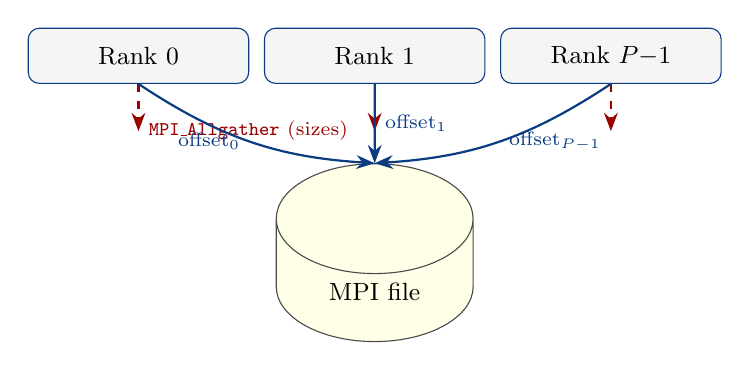
\begin{tikzpicture}[
    rank/.style  = {rectangle, rounded corners, draw=pgsdblue, fill=codebg,
                    minimum width=2.8cm, minimum height=0.7cm, font=\small},
    disk/.style  = {cylinder, draw=pgsdgray, fill=yellow!10,
                    shape border rotate=90, minimum height=1.5cm,
                    minimum width=2.5cm, font=\small},
    arrow/.style = {-Stealth, thick, pgsdblue},
    gather/.style= {-Stealth, thick, red!60!black, dashed},
]

  \node[rank] (r0) at (0,0)    {Rank 0};
  \node[rank] (r1) at (3,0)    {Rank 1};
  \node[rank] (rn) at (6,0)    {Rank $P{-}1$};
  \node[disk] (file) at (3,-3) {MPI file};

  % Allgather
  \draw[gather] (r0.south) -- ++(0,-0.6)
      node[right,font=\scriptsize,text=red!60!black]
        {\code{MPI\_Allgather} (sizes)};
  \draw[gather] (r1.south) -- ++(0,-0.6);
  \draw[gather] (rn.south) -- ++(0,-0.6);

  % Individual writes
  \draw[arrow] (r0.south) to[bend right=15]
      node[left,font=\scriptsize]{offset$_0$} (file.north);
  \draw[arrow] (r1.south) --
      node[right,font=\scriptsize]{offset$_1$} (file.north);
  \draw[arrow] (rn.south) to[bend left=15]
      node[right,font=\scriptsize]{offset$_{P-1}$} (file.north);

\end{tikzpicture}
\caption{Each MPI rank writes its particle partition to a pre-computed file
         offset via \code{MPI\_File\_write\_at}.  The offsets are derived
         from an \code{MPI\_Allgather} of buffer sizes on rank~0.}
\label{fig:mpi-write}
\end{figure}

\subsection{Index and namelist management}

Index entries and the namelist are maintained exclusively on rank~0:

\begin{itemize}[noitemsep]
  \item \textbf{Namelist:} a hash map (\code{pgsd\_name\_id\_map}) allocated
        only on rank~0.  When a new chunk name is first seen, rank~0 assigns
        it the next available id.
  \item \textbf{Index:} rank~0 holds an in-memory array of
        \code{pgsd\_index\_entry\_t} structs, one per written chunk.  When
        the array fills, it is reallocated and rewritten to the end of the
        file.
  \item At \code{pgsd\_close}, rank~0 writes the final index and namelist
        blocks and updates the header.
\end{itemize}

\subsection{Read sequence}

Reading is currently root-only:

\begin{enumerate}[noitemsep]
  \item Rank~0 calls \code{pgsd\_find\_chunk} (binary search in v2 files).
  \item The index entry (or a NULL sentinel) is broadcast with \code{MPI\_Bcast}.
  \item Rank~0 calls \code{MPI\_File\_read\_at} to read the data.
  \item The data is broadcast with \code{MPI\_Bcast} to all ranks.
\end{enumerate}

\notebox{For analysis (post-processing) workloads, use the pure Python reader
\code{pgsd.pypgsd} from a single process to avoid the MPI collective overhead
of broadcast reads.}

\subsection{Design constraints}

\begin{itemize}[noitemsep]
  \item All API calls that touch the file must be invoked collectively across
        \code{MPI\_COMM\_WORLD}.
  \item Particles are written in \emph{rank order}, not sorted by tag.
        Post-processing code must not assume sorted particle order.
  \item All fields are written every timestep, even unchanged ones.  This
        simplifies the write path but increases file size.
  \item The MPI type macro \code{my\_MPI\_SIZE\_T} is used throughout to
        ensure portability across platforms where \code{size\_t} width varies.
\end{itemize}

% ==========================================================================
\section{Complete Examples}
\label{sec:examples}
% ==========================================================================

\subsection{Convert PGSD to VTK (pgsd2vtu)}

The script \code{test\_pgsd2vtu.py} converts PGSD trajectory files to VTK
unstructured grid format for visualisation in ParaView:

\begin{lstlisting}[style=pgsdPython]
#!/usr/bin/env python3
import sys
sys.path.append('./pgsd-3.2.0/build')

import pgsd.hoomd
import pgsd.fl
import numpy as np
from pyevtk.hl import pointsToVTK as vtk

f = pgsd.fl.open(name=sys.argv[1], mode='r',
                 application='HOOMD-SPH', schema='hoomd',
                 schema_version=[1, 0])
t = pgsd.hoomd.HOOMDTrajectory(f)

for count, snapshot in enumerate(t, start=1):
    pname = sys.argv[1].replace('.gsd', f'_{count:05d}')
    pos   = snapshot.particles.position    # (N, 3)
    rho   = snapshot.particles.density     # (N,)
    p     = snapshot.particles.pressure    # (N,)
    vel   = snapshot.particles.velocity    # (N, 3)
    h     = snapshot.particles.slength     # (N,)

    x = np.ascontiguousarray(pos[:, 0], dtype=np.float64)
    y = np.ascontiguousarray(pos[:, 1], dtype=np.float64)
    z = np.ascontiguousarray(pos[:, 2], dtype=np.float64)

    point_data = {
        'density':  np.ascontiguousarray(rho,  dtype=np.float64),
        'pressure': np.ascontiguousarray(p,    dtype=np.float64),
        'slength':  np.ascontiguousarray(h,    dtype=np.float64),
        'velocity': (np.ascontiguousarray(vel[:, 0], dtype=np.float64),
                     np.ascontiguousarray(vel[:, 1], dtype=np.float64),
                     np.ascontiguousarray(vel[:, 2], dtype=np.float64)),
    }
    vtk(pname, x, y, z, pointData=point_data)
    print(f'Frame {count}: N={snapshot.particles.N}')

f.close()
\end{lstlisting}

\subsection{Parallel write with MPI (C)}

\begin{lstlisting}[style=pgsdC]
#include "pgsd.h"
#include <mpi.h>
#include <stdlib.h>

int main(int argc, char **argv)
{
    MPI_Init(&argc, &argv);
    int rank, size;
    MPI_Comm_rank(MPI_COMM_WORLD, &rank);
    MPI_Comm_size(MPI_COMM_WORLD, &size);

    pgsd_handle_t *h;
    pgsd_open(&h, "parallel_output.gsd",
              "my-parallel-sph", "hoomd",
              PGSD_MAKE_VERSION(1, 0),
              PGSD_OPEN_CREATE | PGSD_OPEN_READWRITE);

    /* Each rank owns N_local particles */
    uint64_t N_total = 1000000;
    uint64_t N_local = N_total / size
                     + (rank < (int)(N_total % size) ? 1 : 0);
    uint32_t N_total_u32 = (uint32_t)N_total;

    float *pos = malloc(N_local * 3 * sizeof(float));
    float *rho = malloc(N_local * sizeof(float));
    /* ... fill pos, rho from simulation state ... */

    /* All ranks must write particles/N collectively (root writes value) */
    pgsd_write_chunk(h, "particles/N", 1, 1, 0,
                     PGSD_TYPE_UINT32, &N_total_u32);

    /* Each rank contributes its own rows at its local offset */
    uint64_t row_offset = 0; /* compute prefix sum across ranks */
    MPI_Exscan(&N_local, &row_offset, 1,
                MPI_UINT64_T, MPI_SUM, MPI_COMM_WORLD);

    pgsd_write_chunk(h, "particles/position",
                     N_local, 3, (uint32_t)row_offset,
                     PGSD_TYPE_FLOAT, pos);
    pgsd_write_chunk(h, "particles/density",
                     N_local, 1, (uint32_t)row_offset,
                     PGSD_TYPE_FLOAT, rho);

    pgsd_end_frame(h);
    pgsd_close(h);

    free(pos);
    free(rho);
    MPI_Finalize();
    return 0;
}
\end{lstlisting}

% ==========================================================================
\section{Changelog}
\label{sec:changelog}
% ==========================================================================

\subsection*{Version 3.2.0}

\begin{itemize}[noitemsep]
  \item Initial public PGSD release, forked from GSD 3.2.0.
  \item Replaced POSIX file I/O with MPI-IO throughout \code{pgsd.c}.
  \item Added SPH data chunks: \chunk{particles/slength},
        \chunk{particles/density}, \chunk{particles/pressure},
        \chunk{particles/energy}, \chunk{particles/auxiliary1--4}.
  \item Root-only index and namelist management with per-rank write buffers.
  \item \code{MPI\_Allgather} offset protocol for concurrent multi-rank writes.
  \item Cython wrapper \code{pgsd.fl} adapted from GSD \code{gsd.fl}.
  \item Pure Python reader \code{pgsd.pypgsd} (read-only, no C required).
  \item \code{pgsd.hoomd} HOOMD trajectory interface with SPH field support.
\end{itemize}

% ==========================================================================
\section{License}
\label{sec:license}
% ==========================================================================

Copyright \copyright\ 2016--2023 The Regents of the University of Michigan.\\
Modifications copyright \copyright\ 2023 David Krach, University of Stuttgart.

Redistribution and use in source and binary forms, with or without
modification, are permitted provided that the following conditions are met:

\begin{enumerate}
  \item Redistributions of source code must retain the above copyright notice,
        this list of conditions and the following disclaimer.
  \item Redistributions in binary form must reproduce the above copyright
        notice, this list of conditions and the following disclaimer in the
        documentation and/or other materials provided with the distribution.
\end{enumerate}

THIS SOFTWARE IS PROVIDED BY THE COPYRIGHT HOLDERS AND CONTRIBUTORS ``AS IS''
AND ANY EXPRESS OR IMPLIED WARRANTIES, INCLUDING, BUT NOT LIMITED TO, THE
IMPLIED WARRANTIES OF MERCHANTABILITY AND FITNESS FOR A PARTICULAR PURPOSE ARE
DISCLAIMED.

% ==========================================================================
\section*{Credits}
% ==========================================================================

\textbf{PGSD} was developed by:\\
David Krach, Institute of Applied Mechanics,
University of Stuttgart.

and contributors listed on GitHub.

\end{document}
